\documentclass{homework}
% \usepackage{graphicx} % Required for inserting images
\usepackage{amsmath}
\usepackage{gensymb}
\usepackage{subfig}
\usepackage{float}

\class{ECEN 5738}
\title{Homework 2}
\author{Sean Jennings}
\date{February 7, 2024}

\begin{document}
\maketitle

\section{Problem 1}
To see is $\Omega$ is an invariant set, we verify that $n(x)^T f(x)$
is nonpositive along the border of the set. Along the border $x_1=1$,
the normal vector is $n = \mat{1 & 0}^T$ and we have:
\begin{equation*}
    n^T f(\mat{1 \\ x_2}) = f_1(\mat{1 \\ x_2}) = 1 \cdot (0) \cdot (\alpha(1 - x_2) + 1) = 0
\end{equation*}
Along the border $x_1=0$, the normal vector is $n = \mat{-1 & 0}^T$ so that
for $x_2\in\R$
\begin{equation*}
    n^T f(\mat{0 \\ x_2}) = -f_1(\mat{0 \\ x_2}) = 0 \cdot (1) \cdot (\alpha(1 - x_2))
        = 0
\end{equation*}
Thus, no trajectory of the given system can exit $\Omega$, making it invariant.

\section{Problem 2}
\begin{letterenum}
\item We look at the derivative of $E$ w.r.t. time:
\begin{align*}
    \frac{dE}{dt}(x) &= \nabla_x E^T \dot{x} \\
        &= \nabla_x E^T f(x) \\
        &= \mat{\frac{d\Psi(p)}{dp} & m\dot{p}} \mat{\dot{p} \\ -1/m \phi(p)} \\
        &= \mat{\phi(p) & m\dot{p}} \mat{\dot{p} \\ -1/m \phi(p)} \\
        &= \phi(p) \dot{p} - \phi(p) \dot{p} = 0
\end{align*}
Thus, $E$ does not change over time and is conserved along each trajectory.

\item We recall that $\nabla_x E$ is orthogonal to the level set
$S = \{z\in\R^2: E(z) = c\}$, for $c\in\R$. For if $g: \R \to S$ is some function
which traverses the level set we have:
\begin{equation*}
    E(g(s)) = c
\end{equation*}
and \begin{equation*}
    \nabla_x E^T(g(s)) \frac{dg}{ds}(s) = 0
\end{equation*}
Since $dg/ds$ is tangent to $S$, this implies $\nabla_x E$ is orthogonal to $S$.

Thus, $E$ is a conserved quantity implies that the levels set of $E$ are invariant.
To see this, take any $z\in S$ along the boundary of $S$. Its normal vector
$n(z)$ satifies the following:
\begin{equation*}
    n(z)^T f(z) = \nabla_x E(z)^T \dot{z} = \frac{dE}{dt}(z) = 0
\end{equation*}
\end{letterenum}

\section{Problem 3}
There will be an equilibrium point $\mat{x_1^* & x_2^*}^T$ in the (open) positive
orthant $\R_{>0}^2$ when the second term in each of the system equations is 0.
That is:
\begin{equation*}
    K_1 - x_1^* - \beta_{12} x_2^* = 0
\end{equation*}
and 
\begin{equation*}
    K_2 - x_2^* - \beta_{21} x_1^* = 0
\end{equation*}
which is equivalent to the matrix equation:
\begin{equation*}
    \mat{
        1 & \beta_{12} \\
        \beta_{21} & 1
    } \mat{x_1^* \\ x_2^*} = \mat{
        K_1 \\ K_2
    }
\end{equation*}

If $\beta_{12} \cdot \beta_{21} = 1$, then the equilibrium points are contained
by the set $S = \{[x_1, x_2]\in\R^2: x_2 = -\beta_{21} x_1\}$.
However, this implies $x_1$ and $x_2$ have opposite signs, and thus are not
in $\R_{>0}^2$.

Consider $\beta_{21} \cdot \beta_{12} \neq 1$. Then, we can solve for
the equilibrium point:
\begin{align*}
    \mat{x_1^* \\ x_2^*} &= \mat{
        1 & \beta_{12} \\
        \beta_{21} & 1
    }^{-1} \mat{K_1 \\ K_2} \\
    &= \frac{1}{D} \mat{
        1 & -\beta_{12} \\
        -\beta_{21} & 1
    }
\end{align*}
where $D = 1 - \beta_{12} \beta_{21}$.
So for the eq. point to be in $\R_{>0}^2$, we must have:
\begin{align}
    x_1^* = \frac{1}{D} (K_1 - \beta_{12} K_2) > 0 \label{eq:x1}\\
    x_2^* = \frac{1}{D} (K_2 - \beta_{21} K_1) > 0 \label{eq:x2}
\end{align}

We will show that the inequality
\begin{equation}
    (K_1 - \beta_{12}K_2)(K_2 - \beta{21} K_1) > 0
    \label{eq:ineq-condition}
\end{equation}
is a necessary and sufficient condition for equations (\ref{eq:x1}) and
(\ref{eq:x2}) to hold.

In the forward case, if (\ref{eq:ineq-condition}) holds, then both terms,
$K_1 - \beta_{12} K_2$ and $K_2 - \beta_{21} K_1$, are either strictly
positive or strictly negative. If they are strictly positive,
\begin{equation*}
    K_1 - \beta_{12} K_2 > 0 \qquad K_2 - \beta_{21}K_1 > 0
\end{equation*}
then, rearranging terms, we have
\begin{align*}
    &\beta_{12} < \frac{K_1} K_2 < \frac{1}{\beta{21}} \\
        &\Rightarrow D = 1 - \beta_{12}\beta_{21} > 0 \\
        &\Rightarrow x_1^*, x_2^* > 0.
\end{align*}
Similarly, if both terms are strictly negative, by a similar argument
we find $D<0$ which places $x_1^*, x_2^*$ in the positive orthant.

In the backward case, multiplying equations (\ref{eq:x1}) and (\ref{eq:x2})
implies (\ref{eq:ineq-condition}) since $1/D^2>0$. Thus, (\ref{eq:ineq-condition})
is also a necessary condition.

Thus, another positive quadrant equilibrium position exists if and only if
(\ref{eq:ineq-condition}) and $\beta_{12} \cdot \beta_{12} \neq 1$ both hold.


\section{Problem 4}
We will show that $\mathcal{O}_\beta$ satisfies the conditions of Poincare-Bendixson,
for each $\beta >0$ and therefore contains a periodic orbit.

The gradient of $V$ is given by:
\begin{equation*}
    \nabla V(x) = \mat{c - d / x_1 \\ b - a / x_2}
\end{equation*}
So, $V$ is a conserved quantity, since
\begin{align*}
    \frac{dV}{dt} &= \nabla V(x(t)) \dot{x}(t) \\
        &= \nabla V(x(t)) f(x(t)) \\
        &= (c - d/x_1)(a - bx_2)x_1 + (b - a/x_2)(cx_1 - d)x_2 \\
        &= (cx_1 - d) (a - bx_2) - (a - bx_2) (cx_1 - d) \\
        &= 0.
\end{align*}
Therefore, $\mathcal{O}_\beta$, the level sets of $V$, are positively invariant.
Furthermore, $\mathcal{O}_\beta$ does not contain an equilibrium point for $\beta>0$
since
the only equilibrium points are $x_1^* = [0, 0]^T$ and $x_2^* = [d/c, a/b]^T$.
$V$ is not defined at $x_1^*$ so $x_1^*$ is not in any of its level sets. We
have $V(x_2^*) = 0$ so $x_2^*$ is only in the level set with $\beta=0$.

It remains to be shown the $\mathcal{O}_\beta$ is closed and bounded.
We divide $V$ into two functions $V_1,V_2: \R_{>0} \to \R_{\geq>0}$ with
\begin{equation*}
    V_1(x_1) = cx_1 - d\ln x_1 + d(1 - \ln(d/c))
\end{equation*}
and
\begin{equation*}
    V_2(x_2) = bx_2 - a\ln x_2 + a(1 - \ln(a/b))
\end{equation*}
such that $V([x_1, x_2]) = V_1(x_1) + V_2(x_2)$. We note that since the negative
$\ln$ term in $V_1$ decreases logarithmically, $V_1$ can be lower bounded by
a function of the form $f(x) = mx - b + \beta$ for some $m,b\in\R$, with slope
$m<c$ and sufficiently large $b$.  Since $V_2(x_2)$ is nonnegative, for each
$[x_1, x_2] \in\mathcal{O}_\beta$, we have
\begin{equation*}
    m x_1 - b + \beta \leq V_1(x_1) \leq V_1(x_1) + V_2(x_2) = \beta.
\end{equation*}
Thus, $x_1$ has bounds:
\begin{equation*}
    0 < x_1 \leq \frac{b}{m}
\end{equation*}
By symmetry, $x_2$ is also bounded. Therefore, $\mathcal{O}_\beta$ is compact.

Figure \ref{fig:prob4} shows the vector field and trajectories which confirms
the existence of periodic orbits.

\begin{center}
    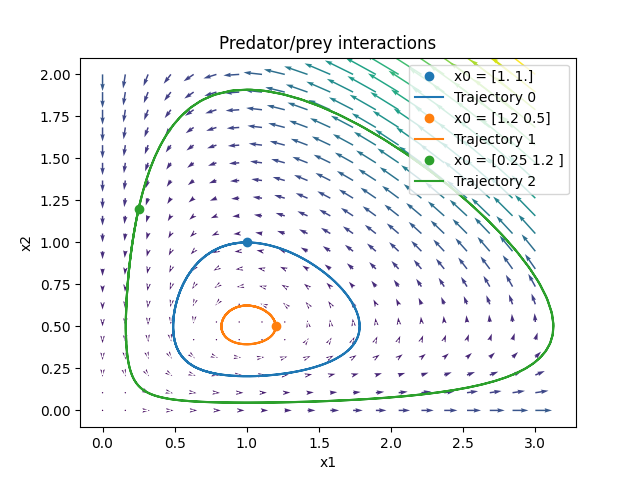
\includegraphics[width=0.8\linewidth]{Images/pred-prey.png}
    \captionof*{figure}{Vector field and State Trajectories for Problem 4}
    \label{fig:prob4}
\end{center}


\section{Problem 5}
\begin{letterenum}
\item The divergence is given by:
\begin{equation*}
    (\nabla \cdot f) = \frac{\delta f_1}{\delta x_1} + \frac{\delta f_2}{\delta x_2}
        = (1 + 6x_1) + (1 + 6x_2) = 2 + 6 (x_1 + x_2)
\end{equation*}
For $x_1,x_2>0$, we have $\nabla \cdot f > 0$ so no limit cycles can occur
over this region.

\item We will show that a limit cycle must exist in the region around
$r=1$. Let $M = \{(x, y) \in\R^2: r_{min} \leq \sqrt{x^2 + y^2} \leq r_{max}\}$
for some $0 < r_{min} < r_{max}$.
If $\dot{r} \leq 0$ along the outer boundary and $\dot{r} \geq 0$ along the inner
boundary, then $M$ is positively invariant.

Along the outer boundary we have:
\begin{equation*}
    \dot{r} = r_{max}(1 - r_{max}^2) + 1/3 r_{max}\sin \theta \leq 0.
\end{equation*}
Since $r_{max} > 0$ and $\sin \theta$ has a maximum of 1, we see the previous equation
holds when
\begin{equation*}
    1 - r_{max}^2  + 1/3 \leq 0
\end{equation*}
so if we take $r_{max} \geq \sqrt{4/3}$, then all trajectories move inwards.

Similarly along the outer boundary we have:
\begin{equation*}
    \dot{r} = r_{min}(1 - r_{min}^2) + 1/3 r_{min}\sin \theta \geq 0.
\end{equation*}
This time, we are interested in the minimum value of $\sin \theta$ which is -1. So,
\begin{equation*}
    1 - r_{min}^2 - 1/3 \geq 0
\end{equation*}
and for any $r_{min} \leq \sqrt{2/3}$ the trajectories move outwards and $M$ is
invariant.

Clearly, $M$ is also compact. Since $\dot{\theta} = -1$, no equilibrium points
exist for $r>0$. Therefore, by Poincare-Bendixson a periodic orbit must exist
within $M$.

\section{Problem 6}
\begin{enumerate}
\item Defining $f: \R^2 \to \R^2$ to be $f(x) = Ax$, the divergence of $f$
for all $x \in \R^2$ is
\begin{equation*}
    \frac{\delta f_1}{\delta x_1}(x) + \frac{\delta f_1}{\delta x_1}(x) = 2\alpha,
\end{equation*}
and is therefore constant and nonzero (for $\alpha \neq 0$). Thus, by
Bendixson's Theorem, the plane $\R^2$ (which is a closed and connected set)
has not limit cycles.

\item Consider the set
\begin{equation*}
    M_r = \{x_1, x_2 \in \R| x_1^2 + x_2^2 = r^2\}
\end{equation*}
for some $r>0$.

Then, for all $x_1,x_2\in M_r$, the vector $n(x) = \mat{x_1 & x_2}^T$ is orthogonal
to $M_r$ and we have
\begin{align*}
    n(x)^T f(x) &= \mat{x_1 & x_2} \mat{0 & \beta \\ -\beta & 0} \mat{x_1 \\ x_2} \\
        &= \mat{x_1 & x_2} \mat{\beta x_2 \\ -\beta x_1} \\
        &= \beta(x_1 x_2 - x_1 x_2) = 0.
\end{align*}
Therefore, $M_r$ is invariant. Also, it does not contain equilibrium points
(only the origin is an equilibrium point since the system is linear).
So it must contain a periodic orbit.

However, this periodic orbit is not isloated since given $\epsilon > 0$,
the set $S = \{x\in\R^2: \text{dist}(x, M_r) < \epsilon\}$ contains
both $M_{r+\delta}$ for any $|\delta| < \epsilon$.
$M_{r+\delta}$ also contains a periodic orbit and it is disjoint
from $M_r$, so $M_{r+\delta}$ represents a distinct limit cycle close to
to $M_r$.

Since a unique periodic orbit $M_r$ exists for every $r>0$, the
number of periodic orbits is infinite.

\end{enumerate}


\end{letterenum}













\end{document}
